\chapter{Architektura systemu}

Założeniem projektu było stworzenie algorytmu weryfikacji modelowej w oparciu o własności LTL dla języka Alvis w środowisku rozproszonym.


\section{Alvis}

Alvis to język formalny, którego celem jest dostarczenie elastyczności w modelowaniu systemów współbieżnych i czasu rzeczywistego wraz z możliwością weryfikacji opartej o metody formalne.
Jego nazwa pochodzi od połączenia słów \textbf{al}gebra i \textbf{vis}ual.
To łatwy w użyciu dla inżynierów formalny język modelowania.
Oferuje także język wizualny do projektowania struktur.
Za pomocą Alvisa modelować można systemy współbieżne, czasu rzeczywistego, wbudowane oraz rozproszone.

Model Alvisa to system agentów, który zazwyczaj działają współbieżnie, komunikują się między sobą, konkurują o współdzielone zasoby itp.
Agenty dzielą się na aktywne i pasywne.
Zachowanie każdego z nich definiuje się w warstwie kodu, którego konstrukcje przypominają języki wysokiego poziomu.

% TODO kilka zdan o modelu, dla ktorego jest weryfikacja
% model systemu to zbior agentow, ktore odpowiadaja dzialaniu aplikacji buildera
% w ich sklad wchodzi m.in. stan heurystyki przeszukiowania BFS, cassandry, czy opisu grafu
% Dla tego modelu tworzone będą formuły LTL, które powinien spełnić.


\section{System rozproszony}

Architektura systemu została zaplanowana tak, aby wydzielić funkcjonalności do odseparowanych aplikacji.
Całość składa się z 3 programów oraz bazy danych.
Jej schemat ogólny został przedstawiony na rys. \ref{fig:system_overview}.

\begin{figure}[h]
    \centering
    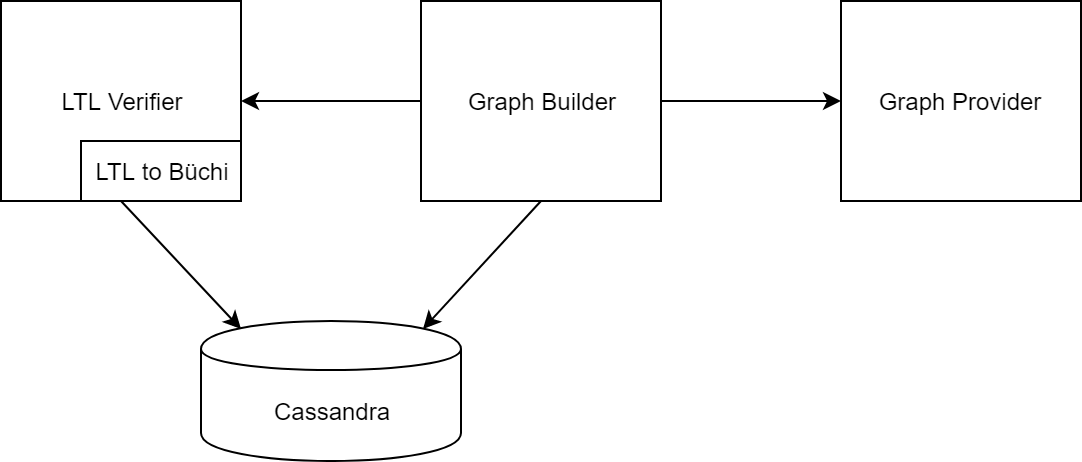
\includegraphics[width=\linewidth,keepaspectratio]{img/system_overview.png}
    \caption{Schemat ogólny systemu.}
    \label{fig:system_overview}
\end{figure}

Pierwszym elementem jest \textit{Graph Provider} (\textbf{GP}).
Spełnia on dwa zadania.
Pierwsze z nich to dostarczanie wszystkich osiągalnych tranzycji dla danego stanu.
Drugie umożliwia otrzymanie stanów dla zadanej tranzycji, które można odwiedzić z wybranego stanu źródłowego.
Serwis ten enkapsuluje działanie całej domeny.
Jako jedyny dostarcza dane, dzięki którym da się zbudować całą przestrzeń stanów.
GP spełnia prosty interfejs przedstawiony w listingu \ref{lst:graph_provider_interface}.

\begin{minipage}{\linewidth}
\begin{lstlisting}[caption={Interfejs implementowany przez GP.},captionpos=b,label={lst:graph_provider_interface}]

  public interface GraphProvider {
    Collection<Transition> allTransitionFromState(SystemState from);

    Collection<SystemState> allReachableStates(SystemState from,
                                               Transition through);
  }
\end{lstlisting}
\end{minipage}

\textit{LTL Verifier} (\textbf{LV}) to główna serwerowa aplikacja zajmująca się weryfikacją modelową i zawiera główną część tego algorytmu.
Konwertuje ona także formuły LTL do automatów Büchiego.
Napisana została w języku Java z wykorzystaniem frameworka Spring.
Interfejs implementowany przez LV opisuje listing \ref{lst:ltl_verifier_interface}.

\begin{lstlisting}[caption={Interfejs implementowany przez LV.},captionpos=b,label={lst:ltl_verifier_interface}]

  public interface LtlVerifier {
    VerificationId createVerificationJob(VerificationInit verificationInit);

    VerificationResult newStates(NewStates newStates,
                                 VerificationId id);

    VerificationResult finish(VerificationId id);
  }
\end{lstlisting}

\textit{Graph Builder} (\textbf{GB}) spełnia rolę serca systemu.
To centrum sterowania, które inicjuje zapytania do pozostałych aplikacji.
Zarządza eksploracją kolejnych stanów, a także wysyła je do weryfikacji.
Zarówno GB jak i LV komunikują się z bazą danych (Cassandra), aby czytać i zapisywać stany czy tranzycje.
Komunikacja między GB a GP zachodzi za pomocą Apache Thrift, wykorzystując binarny protokół przesyłając dane siecią.
Zapytania GB do LV realizowane są poprzez protokół HTTP w formacie JSON.

% TODO dopisać o celach i możliwościach architektury, może diagram z wyszczególnionymi protokołami komunikacji
